%TypeInferencing.tex

%Type Inferencing Rules.

The type system for KerML and thus SysML is known to be unsafe.  That means elements can be used inappropriately leading to avoidable design error.

This section defines type inferencing rules for KerML Core Types and Features which are generalizable to elements derived from them.

Object-oriented languages derive much of their potential for code reuse from inclusion polymorphism.  That means elements may be considered to have multiple types base on inheritance.  Elements of a specialized types are also members of their generalizations.

Let $T$, $U$, $V$, $X$, and $W$ be types, with possible subscripts.

Let $f$, $g$, and $h$ be feature labels.

Let $a$ be an element of type.

The rules below rely on two distinct relationships between types: \emph{specializes} (KerML's
ordinary \texttt{:>}, meaning $T$'s instances are a subset of $U$'s instances) and a second, weaker
relationship used starting with the co-variant feature redefinition rule below, \emph{matches}. $W$
\emph{matches} $T$ when $W$'s
declaration reuses $T$'s owned features, possibly redefining one or more of them -- a purely
structural fact about the declaration, not by itself a guarantee that $W$'s instances are a subset of
$T$'s. Matching licenses feature redefinition; specialization between a redefining type and what it
redefines is only available once the redefinition's variance is actually checked. This split follows
Abadi and Cardelli's \emph{A Theory of Objects}\cite{theory-of-objects}, which distinguishes \emph{subtyping} from
\emph{matching} for exactly this reason: treating matching as if it were automatically subtyping --
i.e., unconstrained covariant feature redefinition -- is a known source of unsoundness in
object-oriented type systems (nothing would then stop, say, a \texttt{DataValue}-typed feature from
being redefined into an unrelated \texttt{Apple}), and was, historically, unconstrained in KerML
itself. The full formal treatment -- \texttt{Matches} and the derivation of specialization from it,
\texttt{MATCH-SPEC} -- is given in \S\ref{sec:match}, after the rules that motivate it.

\section{Specialization Transitivity}
If T specializes U and U specializes V then T specializes V.

\begin{restatable}{definition}{TRANS}~\blTitle{TRANS}~
  Define specialization transitivity.
\begin{align}
\inference
{T~\texttt{:>}~U  ~\wedge~U~\texttt{:>}~V}
%---------------------------------
{T~\texttt{:>}~V}
\label{eq:df-trans}\tag{df-trans}
\end{align}
\end{restatable}

\pn \texttt{TRANS} was book-original with no counterpart in \texttt{Core.lean} until 2026-09-09:
\texttt{Specializes} (\ref{Specializes}) had no transitivity law of its own --
\texttt{df\_specializes} (\ref{df_specializes}) only relates \texttt{Specializes} to \emph{extension}
containment (\texttt{Cs} $\subseteq$ \texttt{Cg}), which composes freely into \texttt{Cs}
$\subseteq$ \texttt{Ch} across two steps but says nothing about whether \texttt{Specializes ts th}
itself holds, since \texttt{Specializes} is only related to extension-subset by that one-way
implication, not defined as it. Added as a field of \texttt{CoreDesignModel} (\ref{CoreDesignModel})
to close the gap.

\begin{restatable}{leandefinition}{TRANSLean}~\leanTitle{TRANS}~ Define specialization transitivity
in Lean. Proven vacuously in the trivial witness, same treatment as \texttt{df\_specializes}
(\texttt{Specializes := fun \_ \_ => False} makes the hypothesis unconstructible).

\texttt{~~TRANS : $\forall$ \{T U V : Element\}, Specializes T U $\to$ Specializes U V $\to$}

\texttt{~~~~Specializes T V}
\label{TRANS}
\end{restatable}

\section{Subsumption}
If $a$ has type $T$ and $T$ specializes $V$, then $a$ also has type $V$.
\begin{restatable}{definition}{SUBS}~\blTitle{SUBS}~  
  Define subsumption.  
\begin{align}
\inference
{T~\texttt{:>}~V ~\wedge~a \in T}
%---------------------------------
{a \in V}
\label{eq:df-subs}\tag{df-subs}
\end{align}
\end{restatable}

\pn Unlike \texttt{TRANS} (\ref{TRANS}), \texttt{SUBS} needed no new field in
\texttt{CoreDesignModel} (\ref{CoreDesignModel}) -- it follows directly from
\texttt{df\_specializes} (\ref{df_specializes}), which already gives \texttt{Ct} $\subseteq$
\texttt{Cv}; plain subset-membership finishes it.

\begin{restatable}{leantheorem}{SUBSLean}~\leanTitle{SUBS}~ The book's own \texttt{SUBS}
(\ref{eq:df-subs}), in Lean -- free directly from \texttt{df\_specializes}.

\texttt{\textcolor{leancolor}{theorem} \textcolor{leanyellow}{SUBS} \{T V a : Element\} \{Ct Cv : Set Element\}}

\texttt{~~(hT : (DesignKind.type, T, Ct) $\in$ Design) (hV : (DesignKind.type, V, Cv) $\in$ Design)}

\texttt{~~(hspec : Specializes T V) (ha : a $\in$ Ct) : a $\in$ Cv :=}

\texttt{~~df\_specializes hT hV hspec ha}
\label{SUBS}
\end{restatable}

\section{Add Feature}
If $T$ specializes $U$ by adding feature $f$, and $a$ has type $T$, then $a$ also has type $U$.\footnote{As
formalized, this conclusion ($a \in U$) never mentions $f$ or $V$, so the ``adding feature $f$
typed $V$'' half of the premise plays no role in deriving it -- \texttt{FEAT} is logically the same
rule as \texttt{SUBS} (\ref{eq:df-subs}) above, just with an unused extra hypothesis decorating the
premise. Contrast \texttt{REDEF}/\texttt{REPL} below, whose conclusions genuinely depend on the
added feature.}
\begin{restatable}{definition}{FEAT}~\blTitle{FEAT}~
  Add a feature to specialization.
\begin{align}
\inference
{T~\texttt{:>}~U\{f:V\} ~\wedge~a \in T}
%---------------------------------
{a \in U}
\label{eq:df-feat}\tag{df-feat}
\end{align}
\end{restatable}

\begin{restatable}{leantheorem}{FEATLean}~\leanTitle{FEAT}~ The book's own \texttt{FEAT}
(\ref{eq:df-feat}), in Lean -- reduces to \texttt{SUBS} (\ref{SUBS}) exactly, with the
\texttt{OwnedFeatureTypedBy} hypothesis kept (and named \texttt{\_hf}) only to state the book's
actual compound premise faithfully.

\texttt{\textcolor{leancolor}{theorem} \textcolor{leanyellow}{FEAT} \{T U f V a : Element\} \{Ct Cu : Set Element\}}

\texttt{~~(hT : (DesignKind.type, T, Ct) $\in$ Design) (hU : (DesignKind.type, U, Cu) $\in$ Design)}

\texttt{~~(hspec : Specializes T U) (\_hf : OwnedFeatureTypedBy T f V) (ha : a $\in$ Ct) : a $\in$ Cu :=}

\texttt{~~SUBS hT hU hspec ha}
\label{FEAT}
\end{restatable}

\section{Co-variant Feature Redefinition}
If $T$ specializes $U$ by adding feature $f$ typed by $V$, and $W$ matches $T$ (\ref{Matches},
\S\ref{sec:match}) by redefining feature $f$ to be typed by $X$, and $X$ specializes $V$, and $a$ has
type $W$ then $a$ also has type $T$.\footnote{\texttt{Specializes W T} is \emph{not} assumed here --
it's derived via \texttt{MATCH\_SPEC} (\ref{MATCH_SPEC}, \S\ref{sec:match}) from \texttt{Matches W T}
plus the checked condition \texttt{X:>V}, and only then combined with \texttt{SUBS} (\ref{eq:df-subs})
the way earlier drafts of this rule assumed outright. Before that derivation existed, this rule
accepted \emph{any} declared redefinition as sound, including one whose new feature type bears no
relation to the old one -- e.g. a \texttt{DataValue}-typed feature redefined into an unrelated
\texttt{Apple}. $T$'s own relationship to $U$/$f$/$V$ and $X$'s relationship to $V$ are no longer
inert for this conclusion the way they once were. Contrast \texttt{REPL} below, whose conclusion is
additionally parametrized by the feature-relabeling operation $T(f \downarrow g)$.}
\begin{restatable}{definition}{REDEF}~\blTitle{REDEF}~   Co-variant feature redefinition.
\begin{align}
\inference
{T\texttt{:>}U\{f:V\}~\wedge~W~\texttt{matches}~T\{f:X~\texttt{:>>}~f\}~\wedge~X\texttt{:>}V ~\wedge~a \in W}
%---------------------------------
{a \in T}
\label{eq:df-redef}\tag{df-redef}
\end{align}
\end{restatable}

\begin{restatable}{leantheorem}{REDEFLean}~\leanTitle{REDEF}~ The book's own \texttt{REDEF}
(\ref{eq:df-redef}), in Lean. \texttt{Specializes W T} is no longer a premise -- it's derived via
\texttt{MATCH\_SPEC} (\ref{MATCH_SPEC}) from \texttt{Matches W T} plus the checked
\texttt{Specializes X V}, then fed into \texttt{SUBS} (\ref{SUBS}) exactly as before.

\texttt{\textcolor{leancolor}{theorem} \textcolor{leanyellow}{REDEF} \{T U f V W X a : Element\} \{Ct Cu Cw : Set Element\}}

\texttt{~~(hT : (DesignKind.type, T, Ct) $\in$ Design) (\_hU : (DesignKind.type, U, Cu) $\in$ Design)}

\texttt{~~(hW : (DesignKind.type, W, Cw) $\in$ Design)}

\texttt{~~(\_hspecTU : Specializes T U) (hfTU : OwnedFeatureTypedBy T f V)}

\texttt{~~(hmatchWT : Matches W T) (hfWT : OwnedFeatureTypedBy W f X)}

\texttt{~~(hspecXV : Specializes X V) (ha : a $\in$ Cw) : a $\in$ Ct :=}

\texttt{~~SUBS hW hT (MATCH\_SPEC hmatchWT hfTU hfWT hspecXV) ha}
\label{REDEF}
\end{restatable}

Let $T(f \downarrow g)$ be $T$ with feature label $f$ replaced by $g$.

If $T$ specializes $U$ by adding feature $f$ typed by $V$, and $W$ matches $T$ (\ref{Matches},
\S\ref{sec:match}) by redefining feature $f$ to be $g$ typed by $X$, and $X$ specializes $V$, and $a$
has type $W$ then $a$ also has type $T$ after replacing label $f$ by label $g$.
\begin{restatable}{definition}{REPL}~\blTitle{REPL}~Feature redefinition with label replacement.
\begin{align}
\inference
{T\texttt{:>}U\{f:V\}~\wedge~W~\texttt{matches}~T\{g:X~\texttt{:>>}~f\}~\wedge~X\texttt{:>}V ~\wedge~a \in W}
%---------------------------------
{a \in T(f \downarrow g)}
\label{eq:df-repl}\tag{df-repl}
\end{align}
\end{restatable}

\pn Unlike \texttt{FEAT} and \texttt{REDEF} above, \texttt{REPL} is not a disguised \texttt{SUBS}:
its conclusion is about $T(f \downarrow g)$, a genuinely different thing from $T$, so formalizing it
needed two real additions to \texttt{Core.lean}, not just a faithful restatement of an existing
theorem's premise. \texttt{CoreDesignModel} carries no notion of ``type identity beyond extension'' --
nothing before now distinguished $T$ from a relabeled variant of $T$ except by literally naming a
different \texttt{Element} for it.

\begin{restatable}{leandefinition}{relabelLean}~\leanTitle{relabel}~ Define $T(f \downarrow g)$ in
Lean: a fresh \texttt{Element} naming the relabeled type, built by nesting \texttt{encodePair}
(\ref{encodePair}) twice rather than a new primitive -- \texttt{encodePair} is already proved
injective, so this needs no axiom of its own either.

\texttt{\textcolor{leancolor}{def} \textcolor{leanyellow}{relabel} (T f g : Element) : Element :=}

\texttt{~~encodePair (encodePair T f) g}
\label{relabel}
\end{restatable}

\begin{restatable}{leandefinition}{dfRelabelLean}~\leanTitle{df\_relabel}~ \texttt{relabel}'s
semantic content, as a new field of \texttt{CoreDesignModel} (\ref{CoreDesignModel}) -- a genuine new
modeling commitment, same status as \texttt{TRANS} (\ref{TRANS}): purely renaming a feature label
doesn't change which elements are instances of a type, so $T(f \downarrow g)$ shares $T$'s own
extension.

\texttt{~~df\_relabel : $\forall$ \{T f g : Element\} \{Ct : Set Element\},}

\texttt{~~~~(DesignKind.type, T, Ct) $\in$ Design $\to$ (DesignKind.type, relabel T f g, Ct) $\in$ Design}
\label{df_relabel}
\end{restatable}

\begin{restatable}{leantheorem}{REPLLean}~\leanTitle{REPL}~ The book's own \texttt{REPL}
(\ref{eq:df-repl}), in Lean. Same setup as \texttt{REDEF} (\ref{REDEF}), except \texttt{W}'s own
feature is labeled \texttt{g}, not \texttt{f} -- exactly the case \texttt{MATCH\_SPEC}
(\ref{MATCH_SPEC}) generalizes over (its own \texttt{f}/\texttt{g} may differ), so the
covariance check spans the rename, comparing \texttt{W}'s \texttt{g}-typed \texttt{X} against
\texttt{T}'s \texttt{f}-typed \texttt{V}. Because \texttt{Design} is a general relation, not
asserted functional (an \texttt{Element} could in principle have more than one associated
extension), the conclusion cannot simply claim $T(f \downarrow g)$'s extension \emph{equals}
\texttt{Ct} -- instead it pairs the same \texttt{a $\in$ Ct} fact \texttt{REDEF} proves with
\texttt{df\_relabel}'s own witness that \texttt{Ct} genuinely is one of \texttt{relabel T f g}'s
extensions.

\texttt{\textcolor{leancolor}{theorem} \textcolor{leanyellow}{REPL} \{T U f V W X g a : Element\} \{Ct Cu Cw : Set Element\}}

\texttt{~~(hT : (DesignKind.type, T, Ct) $\in$ Design) (\_hU : (DesignKind.type, U, Cu) $\in$ Design)}

\texttt{~~(hW : (DesignKind.type, W, Cw) $\in$ Design)}

\texttt{~~(\_hspecTU : Specializes T U) (hfTU : OwnedFeatureTypedBy T f V)}

\texttt{~~(hmatchWT : Matches W T) (hfWT : OwnedFeatureTypedBy W g X)}

\texttt{~~(hspecXV : Specializes X V) (ha : a $\in$ Cw) :}

\texttt{~~a $\in$ Ct $\wedge$ (DesignKind.type, relabel T f g, Ct) $\in$ Design :=}

\texttt{~~$\langle$SUBS hW hT (MATCH\_SPEC hmatchWT hfTU hfWT hspecXV) ha, df\_relabel hT$\rangle$}
\label{REPL}
\end{restatable}

\section{Multiple Inheritance}
If $T$ specializes both $U$ and $V$, and $a$ has type $T$, then $a$ also has type $U$ and type $V$.
\begin{restatable}{definition}{MULTI}~\blTitle{MULTI}~Define multiple specialization of two types.   
\begin{align}
\inference
{T\texttt{:>}U,V ~\wedge~a \in T}
%---------------------------------
{a \in U~\wedge~a \in V}
\label{eq:df-multi}\tag{df-multi}
\end{align}
\end{restatable}

\pn \texttt{MULTI} is \texttt{df-multspec} (\ref{eq:df-multspec}) restated elementwise for exactly
two generalizations, matching \texttt{df\_multspec} (\ref{df_multspec}).

\begin{restatable}{leantheorem}{MULTILean}~\leanTitle{MULTI}~ The book's own \texttt{MULTI}
(\ref{eq:df-multi}), in Lean -- free from \texttt{df\_multspec} via ordinary
intersection-membership.

\texttt{\textcolor{leancolor}{theorem} \textcolor{leanyellow}{MULTI} \{T U V a : Element\} \{Ct Cu Cv : Set Element\}}

\texttt{~~(hT : (DesignKind.type, T, Ct) $\in$ Design) (hU : (DesignKind.type, U, Cu) $\in$ Design)}

\texttt{~~(hV : (DesignKind.type, V, Cv) $\in$ Design)}

\texttt{~~(hspecU : Specializes T U) (hspecV : Specializes T V) (ha : a $\in$ Ct) :}

\texttt{~~a $\in$ Cu $\wedge$ a $\in$ Cv :=}

\texttt{~~Set.mem\_inter\_iff .. |>.mp (df\_multspec hT hU hV hspecU hspecV ha)}
\label{MULTI}
\end{restatable}

Let $U_j~j\in 1 .. n$ be types.  If $T$ specializes multiple types, and $a$ has type $T$, then $a$ also
has each of the types specializes by $T$.
\begin{restatable}{definition}{MULTN}~\blTitle{MULTN}~Define multiple specialization of n types.
\begin{align}
\inference
{T\texttt{:>}U_1,\ldots,U_n ~\wedge~a \in T}
%---------------------------------
{a \in U_1~\wedge \cdots \wedge~ a \in U_n}
\label{eq:df-multn}\tag{df-multn}
\end{align}
\end{restatable}

\pn \texttt{MULTN} is exactly \texttt{df-multspec}'s (\ref{eq:df-multspec}) own claimed $n$-ary
generality, restated elementwise -- see \texttt{df\_multspec\_n} (\ref{df_multspec_n}) for why that
generality needed a real new theorem, not just \texttt{df\_multspec} itself.

\begin{restatable}{leantheorem}{MULTNLean}~\leanTitle{MULTN}~ The book's own \texttt{MULTN}
(\ref{eq:df-multn}), in Lean -- proved directly from \texttt{df\_specializes} applied pointwise,
the elementwise unfolding of \texttt{df\_multspec\_n}'s own conclusion via
\texttt{Set.mem\_iInter}.

\texttt{\textcolor{leancolor}{theorem} \textcolor{leanyellow}{MULTN} \{n : $\mathbb{N}$\} \{ts a : Element\} \{Cs : Set Element\}}

\texttt{~~\{tg : Fin n $\to$ Element\} \{Cg : Fin n $\to$ Set Element\}}

\texttt{~~(hs : (DesignKind.type, ts, Cs) $\in$ Design)}

\texttt{~~(hg : $\forall$ i, (DesignKind.type, tg i, Cg i) $\in$ Design)}

\texttt{~~(hspec : $\forall$ i, Specializes ts (tg i)) (ha : a $\in$ Cs) :}

\texttt{~~$\forall$ i, a $\in$ Cg i :=}

\texttt{~~fun i $\Rightarrow$ df\_specializes hs (hg i) (hspec i) ha}
\label{MULTN}
\end{restatable}

\section{Multiple Inheritance with Features}
If $T$ specializes both $U_1$ and $V_1$, \\
$U_1$ specializes $U_2$ by adding feature $f$ typed by $U_3$, and\\
$V_1$ specializes $V_2$ by adding feature $g$ typed by $V_3$, \\
and $f$ is different than $g$, \\
then $T$ specializes both $U_2$ and $V_2$, while adding features $f$ and $g$.
\begin{restatable}{definition}{MULTF}~\blTitle{MULTF}~ Multiple specialization with distinct features.
\begin{align}
\inference
{T\texttt{:>}U_1 , V_1~\wedge~U_1\texttt{:>}U_2\{f:U_3\}~\wedge~V_1\texttt{:>}V_2\{g:V_3\}~\wedge~f \ne g}
%---------------------------------
{T\texttt{:>}U_2 , V_2\{f:U_3 ;~ g:V_3\}}
\label{eq:df-multf}\tag{df-multf}
\end{align}
\end{restatable}

\pn \texttt{MULTF}'s conclusion is compound: \texttt{T:>U\_2,V\_2} (two applications of
\texttt{TRANS}, \ref{TRANS}) \emph{and} that \texttt{T} itself now owns (inherits) $f$/$g$ --
something no earlier rule needed, since \texttt{FEAT}/\texttt{REDEF}/\texttt{REPL} all state
\texttt{OwnedFeatureTypedBy} of the type doing the adding, never propagate it to a further
specializer. That propagation is a genuine new modeling commitment, \texttt{df\_feature\_inherit}:

\begin{restatable}{leandefinition}{dfFeatureInheritLean}~\leanTitle{df\_feature\_inherit}~ A new
field of \texttt{CoreDesignModel} (\ref{CoreDesignModel}), same status as \texttt{TRANS}/
\texttt{df\_relabel}: a directly-owned feature is inherited down every structural match
(\ref{Matches}, \S\ref{sec:match}) -- stated over \texttt{Matches} rather than \texttt{Specializes}
since the §4.9 matching split: feature inheritance is a structural fact about a declaration, not
something that should presuppose the extensional consequence (\texttt{Specializes}) the declaration
may or may not actually earn once redefinition is checked.

\texttt{~~df\_feature\_inherit : $\forall$ \{Z W f X : Element\},}

\texttt{~~~~Matches Z W $\to$ OwnedFeatureTypedBy W f X $\to$ OwnedFeatureTypedBy Z f X}
\label{df_feature_inherit}
\end{restatable}

\begin{restatable}{leantheorem}{MULTFLean}~\leanTitle{MULTF}~ The book's own \texttt{MULTF}
(\ref{eq:df-multf}), in Lean. The \texttt{Specializes} half of the conclusion is two applications of
\texttt{TRANS}; the feature half is two applications of \texttt{df\_feature\_inherit}, fed via
\texttt{matches\_of\_specializes} (\ref{matches_of_specializes}) -- plain, non-redefining
specialization is trivially a match (\S\ref{sec:match}). $f \ne g$
(kept as \texttt{\_hne}, unused) plays no logical role in deriving either half individually -- it
only distinguishes this rule from \texttt{MULTS} below, which merges a \emph{shared} label instead.

\texttt{\textcolor{leancolor}{theorem} \textcolor{leanyellow}{MULTF} \{T U1 U2 U3 V1 V2 V3 f g : Element\}}

\texttt{~~(hspecTU1 : Specializes T U1) (hspecU1U2 : Specializes U1 U2)}

\texttt{~~(hfU1 : OwnedFeatureTypedBy U1 f U3)}

\texttt{~~(hspecTV1 : Specializes T V1) (hspecV1V2 : Specializes V1 V2)}

\texttt{~~(hgV1 : OwnedFeatureTypedBy V1 g V3)}

\texttt{~~(\_hne : f $\ne$ g) :}

\texttt{~~Specializes T U2 $\wedge$ Specializes T V2 $\wedge$}

\texttt{~~~~OwnedFeatureTypedBy T f U3 $\wedge$ OwnedFeatureTypedBy T g V3 :=}

\texttt{~~$\langle$TRANS hspecTU1 hspecU1U2, TRANS hspecTV1 hspecV1V2,}

\texttt{~~~~df\_feature\_inherit (matches\_of\_specializes hspecTU1) hfU1,}

\texttt{~~~~df\_feature\_inherit (matches\_of\_specializes hspecTV1) hgV1$\rangle$}
\label{MULTF}
\end{restatable}

If $T$ specializes both $U_1$ and $V_1$, \\
$U_1$ specializes $U_2$ by adding feature $f$ typed by $U_3$, and\\
$V_1$ specializes $V_2$ by adding feature $f$ typed by $V_3$, \\
then $T$ specializes both $U_2$ and $V_2$, while adding feature $f$ which is typed by both $U_3$ and $V_3$.

\begin{restatable}{definition}{MULTS}~\blTitle{MULTS}~  Multiple specialization with same-label features
\begin{align}
\inference
{T\texttt{:>}U_1 , V_1~\wedge~U_1\texttt{:>}U_2\{f:U_3\}~\wedge~V_1\texttt{:>}V_2\{f:V_3\}}
%---------------------------------
{T\texttt{:>}U_2 , V_2\{f:U_3,V_3\}}
\label{eq:df-mults}\tag{df-mults}
\end{align}
\end{restatable}

\begin{restatable}{leantheorem}{MULTSLean}~\leanTitle{MULTS}~ The book's own \texttt{MULTS}
(\ref{eq:df-mults}), in Lean -- same setup as \texttt{MULTF}, except both branches redefine the
\emph{same} label $f$, so \texttt{T} ends up inheriting $f$ typed by both $U_3$ and $V_3$
simultaneously (the multi-typing a real KerML redefinition merge produces), proved by the identical
\texttt{TRANS}/\texttt{df\_feature\_inherit}-via-\texttt{matches\_of\_specializes} combination.

\texttt{\textcolor{leancolor}{theorem} \textcolor{leanyellow}{MULTS} \{T U1 U2 U3 V1 V2 V3 f : Element\}}

\texttt{~~(hspecTU1 : Specializes T U1) (hspecU1U2 : Specializes U1 U2)}

\texttt{~~(hfU1 : OwnedFeatureTypedBy U1 f U3)}

\texttt{~~(hspecTV1 : Specializes T V1) (hspecV1V2 : Specializes V1 V2)}

\texttt{~~(hfV1 : OwnedFeatureTypedBy V1 f V3) :}

\texttt{~~Specializes T U2 $\wedge$ Specializes T V2 $\wedge$}

\texttt{~~~~OwnedFeatureTypedBy T f U3 $\wedge$ OwnedFeatureTypedBy T f V3 :=}

\texttt{~~$\langle$TRANS hspecTU1 hspecU1U2, TRANS hspecTV1 hspecV1V2,}

\texttt{~~~~df\_feature\_inherit (matches\_of\_specializes hspecTU1) hfU1,}

\texttt{~~~~df\_feature\_inherit (matches\_of\_specializes hspecTV1) hfV1$\rangle$}
\label{MULTS}
\end{restatable}

\section{Multiple Inheritance with Feature Multiplicity}
Let $m_u$ and $m_v$ be feature multiplicities which may be a single natural number or a range of natural numbers with
$m_u\cap m_v$ being those multiplicities in common to both.

If $T$ specializes both $U_1$ and $V_1$, \\
$U_1$ specializes $U_2$ by adding feature $f$ typed by $U_3$ with multiplicity $m_u$, and\\
$V_1$ specializes $V_2$ by adding feature $f$ typed by $V_3$ with multiplicity $m_v$, \\
then $T$ specializes both $U_2$ and $V_2$, while adding feature $f$ with multiplicity being the intersection of the respective multiplicities $m_u$ and $m_v$, which is typed by both $U_3$ and $V_3$.

\begin{restatable}{definition}{MULTM}~\blTitle{MULTM}~
Multiple specialization with same-label features having multiplicities.
\begin{align}
\inference
{T\texttt{:>}U_1 , V_1~\wedge~U_1\texttt{:>}U_2\{f[m_u]:U_3\}~\wedge~V_1\texttt{:>}V_2\{f[m_v]:V_3\}}
%---------------------------------
{T\texttt{:>}U_2 , V_2\{f[m_u\cap m_v]:U_3,V_3\}}
\label{eq:df-multm}\tag{df-multm}
\end{align}
\end{restatable}

Note: if the multiplicities in common between $m_u$ and $m_v$, $m_u\cap m_v$ is empty, the result must be a type error--not multiplicity [0].

\pn Formalized narrower than $m_u$/$m_v$'s fully general ``single number or range'' phrasing: in Lean,
multiplicity is always a range -- an exact multiplicity $k$ is the degenerate range $[k,k]$, so this
loses no generality \texttt{CoreDesignModel} already has. Unlike \texttt{MULTS} above, merging two
ranges is a genuine new commitment, not derivable from \texttt{df\_feature\_inherit} (which only
propagates one fact, unchanged, down a single path):

\begin{restatable}{leandefinition}{dfFeatureInheritRangeMergeLean}~\leanTitle{df\_feature\_inherit\_range\_merge}~
A new field of \texttt{CoreDesignModel} (\ref{CoreDesignModel}), same status as \texttt{TRANS}/
\texttt{df\_relabel}/\texttt{df\_feature\_inherit}: when the same feature label is inherited from two
different ancestors, each with a range multiplicity, the two ranges intersect. \texttt{max l1 l2}
$\le$ \texttt{min u1 u2} (the intersection is nonempty) is a hypothesis, not something the rule
derives -- matching the book's own note above that an empty intersection must be a type error, not
multiplicity \texttt{[0]}. Stated over \texttt{Matches}, same reasoning as
\texttt{df\_feature\_inherit} (\ref{df_feature_inherit}).

\texttt{~~df\_feature\_inherit\_range\_merge : $\forall$ \{Z W1 W2 f X1 X2 : Element\} \{l1 u1 l2 u2 : $\mathbb{N}$\},}

\texttt{~~~~Matches Z W1 $\to$ OwnedFeatureTypedByRange W1 f X1 l1 u1 $\to$}

\texttt{~~~~Matches Z W2 $\to$ OwnedFeatureTypedByRange W2 f X2 l2 u2 $\to$}

\texttt{~~~~max l1 l2 $\le$ min u1 u2 $\to$}

\texttt{~~~~OwnedFeatureTypedByRange Z f X1 (max l1 l2) (min u1 u2) $\wedge$}

\texttt{~~~~OwnedFeatureTypedByRange Z f X2 (max l1 l2) (min u1 u2)}
\label{df_feature_inherit_range_merge}
\end{restatable}

\begin{restatable}{leantheorem}{MULTMLean}~\leanTitle{MULTM}~ The book's own \texttt{MULTM}
(\ref{eq:df-multm}), in Lean -- same setup as \texttt{MULTS} (\ref{MULTS}), except the inherited
feature's multiplicity is a range on both branches, and the conclusion's multiplicity is their
intersection. Fed via \texttt{matches\_of\_specializes} (\ref{matches_of_specializes}), same reasoning
as \texttt{MULTF}/\texttt{MULTS}.

\texttt{\textcolor{leancolor}{theorem} \textcolor{leanyellow}{MULTM} \{T U1 U2 U3 V1 V2 V3 f : Element\} \{lu uu lv uv : $\mathbb{N}$\}}

\texttt{~~(hspecTU1 : Specializes T U1) (hspecU1U2 : Specializes U1 U2)}

\texttt{~~(hfU1 : OwnedFeatureTypedByRange U1 f U3 lu uu)}

\texttt{~~(hspecTV1 : Specializes T V1) (hspecV1V2 : Specializes V1 V2)}

\texttt{~~(hfV1 : OwnedFeatureTypedByRange V1 f V3 lv uv)}

\texttt{~~(hoverlap : max lu lv $\le$ min uu uv) :}

\texttt{~~Specializes T U2 $\wedge$ Specializes T V2 $\wedge$}

\texttt{~~~~OwnedFeatureTypedByRange T f U3 (max lu lv) (min uu uv) $\wedge$}

\texttt{~~~~OwnedFeatureTypedByRange T f V3 (max lu lv) (min uu uv) :=}

\texttt{~~$\langle$TRANS hspecTU1 hspecU1U2, TRANS hspecTV1 hspecV1V2,}

\texttt{~~~~(df\_feature\_inherit\_range\_merge (matches\_of\_specializes hspecTU1) hfU1}

\texttt{~~~~~~(matches\_of\_specializes hspecTV1) hfV1 hoverlap).1,}

\texttt{~~~~(df\_feature\_inherit\_range\_merge (matches\_of\_specializes hspecTU1) hfU1}

\texttt{~~~~~~(matches\_of\_specializes hspecTV1) hfV1 hoverlap).2$\rangle$}
\label{MULTM}
\end{restatable}

\section{Contravariant Expression Specialization}\label{sec:contra}

Let $I \rightarrow R$ represent an expression with input $I$ returning result $R$.
\begin{restatable}{definition}{CONTRA}~ \blTitle{CONTRA}~
  Define contravariant specialization of expressions and functions.  
\begin{align}
\inference
{S_1~\texttt{:>}~T_1  ~\wedge~T_2~\texttt{:>}~S_2}
%---------------------------------
{T_1 \rightarrow T_2~\texttt{:>}~S_1 \rightarrow S_2}
\label{eq:df-contra}\tag{df-contra}
\end{align}
\end{restatable}

\pn \texttt{CONTRA} is the only rule in this chapter about a relationship \emph{between two
function/expression types themselves}, rather than instance membership -- \texttt{CoreDesignModel}
has no notion of function types at all otherwise, so formalizing it needed genuinely new
machinery, the same kind of addition as \texttt{TRANS} (\ref{TRANS}).

\begin{restatable}{leandefinition}{arrowLean}~\leanTitle{arrow}~ Define $I \rightarrow R$ in Lean: a
fresh \texttt{Element} naming the arrow type, built from \texttt{encodePair} (\ref{encodePair})
rather than a new primitive, same treatment as \texttt{relabel} (\ref{relabel}). Its semantic
content (contravariant specialization) is \texttt{CONTRA} itself, not this \texttt{def}, which is
pure naming.

\texttt{\textcolor{leancolor}{def} \textcolor{leanyellow}{arrow} (I R : Element) : Element :=}

\texttt{~~encodePair I R}
\label{arrow}
\end{restatable}

\begin{restatable}{leandefinition}{CONTRALean}~\leanTitle{CONTRA}~ A new field of
\texttt{CoreDesignModel} (\ref{CoreDesignModel}), same status as \texttt{TRANS}: specialization of
arrow types is contravariant in the input, covariant in the result. Nothing about plain
\texttt{Specializes} on the components could ever derive a fact about \texttt{Specializes} on the
constructed \texttt{arrow} types without a field like this one.

\texttt{~~CONTRA : $\forall$ \{S1 T1 T2 S2 : Element\},}

\texttt{~~~~Specializes S1 T1 $\to$ Specializes T2 S2 $\to$ Specializes (arrow T1 T2) (arrow S1 S2)}
\label{CONTRA}
\end{restatable}

$T_1 \rightarrow T_2$ can be used in place of $S_1 \rightarrow S_2$ because: \\
$T_1$ is \emph{bigger} than $S_1$ (any input value in $S_1$ will also be in $T_1$), and \\
$T_2$ is \emph{smaller} than $S_2$ (any output value in $T_2$ will also be in $S_2$).

\begin{lstlisting}
S1 :> T1;
T2 :> S2;
expr S {
  in x : S1;
  return y : S2; }
expr T :> S {
  in x : T1 :>> x;
  return y : T2 :>> y; } 
\end{lstlisting}

We want to use $T$ in place of $S$.  Redefinition keeps labels the same.

Because $T_1$ is bigger than $S_1$ when we invoke $T$ as if it was $S$ the input to $S$ will be okay for $T$.
Conversely, $T$ is producing a result in $T_2$ which is bigger than $S_2$ so the output will be okay for $S$.
Figure \ref{fig:contra} depicts these relationships.

\begin{figure}[htbp]
\begin{center}
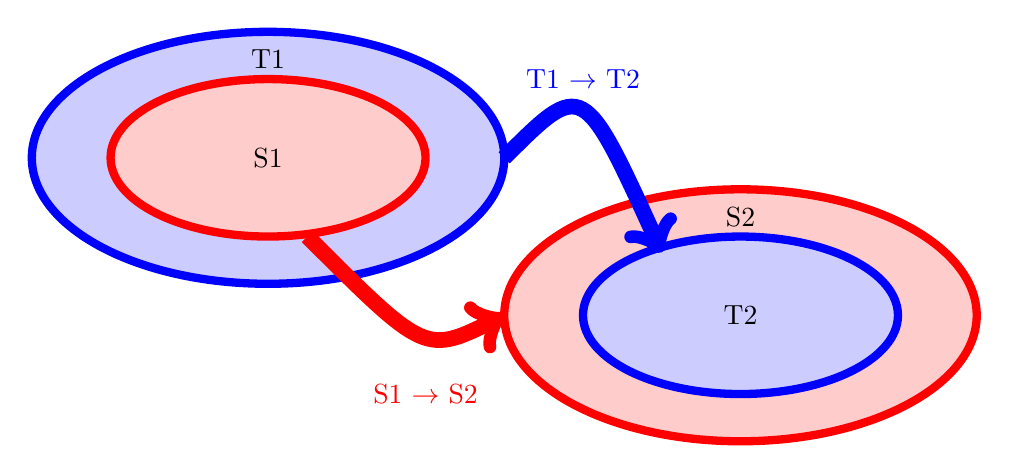
\begin{tikzpicture}[scale=1, line width=3pt]	%%make TiKZ picture
	\filldraw[fill=blue!20!white, draw=blue] (4,4) arc (0:360:3 and 1.6); %circle (4);
	\fill[fill=red!20!white, draw=red] (3,4) arc (0:360:2 and 1);
	\fill[fill=red!20!white, draw=red] (10,2) arc (0:360:3 and 1.6);
	\filldraw[fill=blue!20!white, draw=blue] (9,2) arc (0:360:2 and 1); 
	\draw[color=black] (1,5.25) node {T1};
	\draw[color=black] (1,4) node {S1};
	\draw[color=black] (7,2) node {T2};
	\draw[color=black] (7,3.25) node {S2};
   \draw[red, line width=2mm, arrows= {->}] (1.5,3) .. controls (3,1.5)  .. (4,2);
   \draw[blue, line width=2mm, arrows= {->}] (4,4) .. controls (5,5)  .. (6,2.8);
   \draw[color=blue] (5,5) node {T1 $\rightarrow$ T2};
   \draw[color=red] (3,1) node {S1 $\rightarrow$ S2};
	\end{tikzpicture}
\caption{Contravariant Specialization of Expression}
\label{fig:contra}
\end{center}
\end{figure}

When T is used instead of S, it receives input from S1 which is okay because it's within T1.  Its output in in T2 which is okay because using T instead of S is expecting something in S2 which is bigger than T2.

\section{Matching and Redefinition Safety}\label{sec:match}

\texttt{REDEF} and \texttt{REPL} earlier in this chapter both licensed a redefining declaration by
simply assuming \texttt{Specializes W T} -- that $W$, having redefined a feature of $T$, specializes
$T$. Nothing checked this. A model could declare a \texttt{DataValue}-typed feature redefined into an
unrelated \texttt{Apple}, and this chapter's own rules would still treat the redefining type as a
sound specialization, because \texttt{Specializes W T} was handed in as a premise rather than
established. This is not a hypothetical concern: unconstrained covariant feature redefinition is a
well-known unsoundness in object-oriented type systems (Eiffel's covariant argument typing being the
canonical historical case), and KerML itself originally had no enforcement here.

\pn Abadi and Cardelli's \emph{A Theory of Objects} diagnose exactly this failure mode by splitting
what a single ``inherits from'' relation is being asked to do into two relations: \emph{subtyping}
($\preceq$, \texttt{Specializes} here -- substitutability, the extension-containment guarantee
\texttt{df\_specializes} (\ref{df_specializes}) already gives) and \emph{matching} ($\preceq_\#$,
\texttt{Matches} below -- a purely structural claim: ``has at least these features, possibly
overridden,'' carrying no substitutability guarantee by itself). Redefinition is licensed by matching.
Substitutability is only available once a redefinition's variance is actually checked.

\begin{restatable}{leandefinition}{MatchesLean}~\leanTitle{Matches}~ A new primitive relation on
\texttt{CoreDesignModel} (\ref{CoreDesignModel}), alongside \texttt{Specializes}
(\ref{Specializes}): Abadi/Cardelli's matching ($\preceq_\#$). \texttt{Matches Z W} means ``$Z$'s
declaration reuses $W$'s owned features, each possibly redefined'' -- structural, and carrying none
of \texttt{Specializes}'s extensional weight on its own.

\texttt{~~Matches : Element $\to$ Element $\to$ Prop}
\label{Matches}
\end{restatable}

\begin{restatable}{leandefinition}{matchesOfSpecializesLean}~\leanTitle{matches\_of\_specializes}~ A
new field of \texttt{CoreDesignModel}, same status as \texttt{TRANS} (\ref{TRANS}): ordinary
specialization without any feature redefinition is automatically a (trivial) match --
\texttt{Matches} only becomes strictly weaker than \texttt{Specializes} once redefinition enters the
picture, via \texttt{MATCH\_SPEC} below. This is what lets \texttt{MULTF}/\texttt{MULTS}/\texttt{MULTM}
earlier in this chapter, whose own premises are ordinary \texttt{Specializes}
chains with no redefinition involved, keep feeding \texttt{df\_feature\_inherit}
(\ref{df_feature_inherit})/\texttt{df\_feature\_inherit\_range\_merge}
(\ref{df_feature_inherit_range_merge}) once those are restated over \texttt{Matches}.

\texttt{~~matches\_of\_specializes : $\forall$ \{Z W : Element\}, Specializes Z W $\to$ Matches Z W}
\label{matches_of_specializes}
\end{restatable}

\pn Matching alone still doesn't give substitutability -- that's the whole point. What licenses
\texttt{Specializes W T} for a redefining declaration is a genuinely new checked condition: the
redefined feature's new type must itself specialize the type it replaces.

\begin{restatable}{definition}{MATCHSPEC}~\blTitle{MATCH-SPEC}~ Define specialization derived from
matching plus a checked co-variant feature redefinition.
\begin{align}
\inference
{Z~\texttt{matches}~W~\wedge~W\{f:V\}~\wedge~Z\{g:X\}~\wedge~X~\texttt{:>}~V}
%---------------------------------
{Z~\texttt{:>}~W}
\label{eq:df-matchspec}\tag{df-matchspec}
\end{align}
\end{restatable}

\pn $f$ and $g$ may differ, covering \texttt{REPL}'s renaming case as well as \texttt{REDEF}'s
same-name case. This is a genuine new modeling commitment, same status as \texttt{TRANS}/
\texttt{df\_relabel}/\texttt{df\_feature\_inherit} -- \texttt{Matches} alone carries no extensional
content, so nothing about it could derive a \texttt{Specializes} fact without a field like this one.
Its point is exactly what it rules out: a redefinition whose new feature type does \emph{not}
specialize the old one never lets \texttt{Specializes Z W} be established via this route.

\begin{restatable}{leandefinition}{MATCHSPECLean}~\leanTitle{MATCH\_SPEC}~ The book's own
\texttt{MATCH-SPEC} (\ref{eq:df-matchspec}), as a new field of \texttt{CoreDesignModel}.

\texttt{~~MATCH\_SPEC : $\forall$ \{Z W f g X V : Element\},}

\texttt{~~~~Matches Z W $\to$ OwnedFeatureTypedBy W f V $\to$ OwnedFeatureTypedBy Z g X $\to$}

\texttt{~~~~Specializes X V $\to$ Specializes Z W}
\label{MATCH_SPEC}
\end{restatable}

